\section{Introduction}
Sorting remains one of the most studied problems in computer science due to its central role in data processing.
For decades, the $\Omega(N \log N)$ lower bound for comparison-based algorithms has defined the performance baseline for general-purpose sorting.
While classic algorithms such as QuickSort \cite{10.1093/comjnl/5.1.10} provide flexibility and strong average-case performance while maintaining predictable worst-case behavior, their reliance on comparison operators introduces a large volume of conditional branching.

While these approaches provide acceptable baseline performance, sorting on modern superscalar processors is increasingly dominated by microarchitectural effects such as cache locality, memory bandwidth saturation, and branch misprediction penalties rather than arithmetic complexity \cite{frigoCacheobliviousAlgorithms1999b, wulfHittingMemoryWall1995}.
As a result, minimizing comparisons alone is often insufficient for maximizing throughput on multi-core systems; instead, algorithms must prioritize memory locality and avoid unpredictable branching.

On the other hand, non-comparison sorting algorithms such as radix and counting sort \cite{cormenIntroductionAlgorithms2022} address these limitations by replacing comparison trees with fixed-cost classification passes.
However, they typically depend on strict constraints on data representation, exhibit increased sensitivity to skewed distributions, or incur heavy memory overhead when generalized to arbitrary data types.

\subsection{Motivation: From Comparison Trees to Spatial Classification}
The central observation motivating Adaptive Range Sorting (ARS) is that traditional sorting performance is strongly influenced by the cost of branch-heavy decision trees.
A single branch misprediction on a modern CPU can stall the execution pipeline for 15--20 cycles.
While this overhead is negligible for small datasets, comparison-driven partitioning can introduce substantial pipeline inefficiency at scales involving millions of elements \cite{kaligosiHowBranchMispredictions2006}.

ARS addresses this issue by transforming sorting into a spatial classification problem.
Instead of comparing elements through recursive decision trees, the framework projects data into a monotonic spatial domain using a mapping function $\mathcal{K}$ (formally defined in \cref{sec:methodology}), which enables fixed-cost classification, cache-conscious memory scattering, and reduced dependence on unpredictable branching.

\cref{fig:teaser} illustrates the resulting “Spatial Advantage” across several workload classes.
ARS Aero achieves substantial speedups on high-entropy and complex-type datasets while remaining competitive on low-entropy duplicate-heavy workloads.

\begin{figure*}[t]
\centering
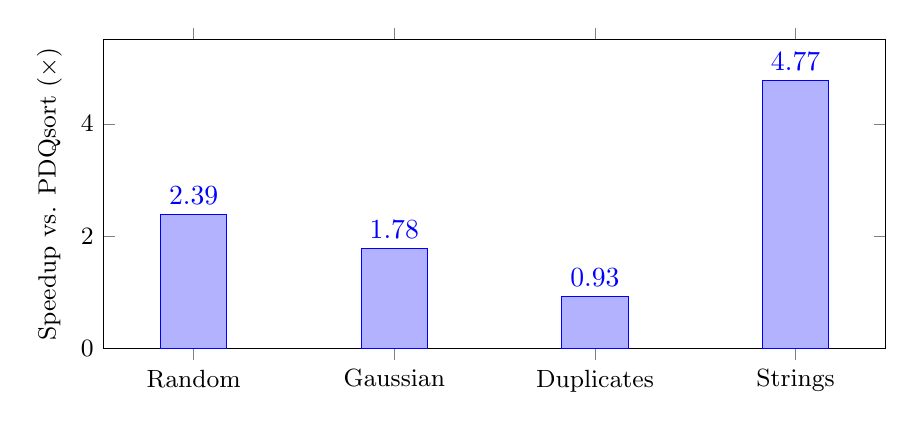
\begin{tikzpicture}
\begin{axis}[
    ybar,
    width=0.95\linewidth, height=5.5cm,
    enlarge x limits=0.15,
    ylabel={Speedup vs. PDQsort ($\times$)},
    symbolic x coords={Random, Gaussian, Duplicates, Strings},
    xtick=data,
    nodes near coords,
    nodes near coords align={vertical},
    ymin=0, ymax=5.5,
    major grid style={dashed, gray!30},
    bar width=24pt,
    fill=teal!70,
    label style={font=\small},
    tick label style={font=\small}
]
\addplot coordinates {(Random, 2.39) (Gaussian, 1.78) (Duplicates, 0.93) (Strings, 4.77)};
\end{axis}
\end{tikzpicture}
\caption{The "Spatial Advantage": ARS Aero Speedup across diverse data domains ($N=10^7$) on i64 datatype and random strings. The framework demonstrates significant gains in high-entropy and complex-type sorting while maintaining competitive parity on low-entropy duplicates.}
\label{fig:teaser}
\end{figure*}

\subsection{Spatial Mapping and Hardware-Conscious Processing}
\textbf{Spatial Mapping} is the core mechanism behind ARS.
By projecting values into a monotonic discrete spatial domain while preserving ordering relationships, ARS transforms sorting into a \textbf{spatial classification} problem. 
This allows the framework to operate through histogramming, prefix-sum partitioning, and contiguous scatter operations rather than comparison-driven recursive branching.

Furthermore, ARS is designed to align these operations with modern hardware behavior.
By emphasizing sequential memory access, cache-resident classification structures, and write-combined scatter phases, ARS prioritizes memory efficiency and instruction reduction over comparison minimization alone.

\subsection{Scientific Contributions}
The scientific contributions of this paper span adaptive classification, streaming consolidation, and hardware-level performance evaluation.
First, we introduce Aero (ARS Gen 6), a quantile-adaptive architecture that utilizes a cache-resident 1024-entry division-free lookup table to improve robustness under skewed and non-uniform distributions.
Unlike traditional range-based approaches, Aero maintains stable classification costs across varying entropy profiles while remaining competitive with state-of-the-art parallel sorters such as IPS4o \cite{axtmannInPlaceParallelSuper2017}.
As illustrated in \cref{fig:teaser}, these gains are particularly pronounced for high-entropy and complex-type workloads, where branch-heavy comparison sorting becomes increasingly memory and prediction bound.

In addition, we introduce ARS Exp D, a streaming architecture based on epoch micro-batching and concurrent spatial consolidation.
Exp D enables sustained high-throughput ingestion with bounded memory growth while reducing the interference between ingestion and background consolidation workloads.

Finally, we provide an extensive hardware-level evaluation of the ARS framework across multiple workload classes and data distributions.
Our analysis examines throughput scaling, cache behavior, branch efficiency, latency stability, streaming interference, and memory-bandwidth limitations on modern multi-core hardware.
The results indicate that spatial classification provides a practical alternative to comparison-driven sorting for hardware-conscious data processing systems.
However, ARS is not intended to universally replace comparison-based sorting algorithms.
Instead, the framework targets high-throughput workloads where classification cost, memory locality, and branch efficiency dominate execution time.
